\documentclass{article}
\usepackage[margin=0.7in]{geometry}
\usepackage{amsmath}
\usepackage{amssymb}
\usepackage{bookmark}
\usepackage{graphicx}
\usepackage{float}

\title{Report for Assignment - 1: CS6370 - \\Information Retrieval}
\author{
Harsh Agarwal\\\texttt{CS15BTECH11019}
\and
Sukrut Rao\\\texttt{CS15BTECH11036}
\and
Vishwak Srinivasan\\\texttt{CS15BTECH11043}
}
\date{}

\begin{document}
\maketitle

\section{Introduction}
\begin{flushleft}
This assignment focused on empirically verifying \textbf{Zipf's Law} and \textbf{Heaps' Law} for two different datasets. Task 1 focused on the verification of the former, while Task 2 focused on the verification of the latter. Task 1 was a bit more involved than Task 2, because of the more text processing that had to be done to satisfy requirements.
\(\newline\)

Some statistics of the datasets: the first dataset (i.e., the dataset in CSV format) contains 32578 documents and the second dataset (i.e., the dataset in JSON format) contains 32912 documents.

\subsection{Pre-processing the datasets}
The main scripts provided work fine on datasets in the CSV format. For this we had to convert the dataset in JSON to CSV format. During this process we found certain parsing errors due to escape characters. These were found in lines \{9045, 9838, 13550, 14553, 16890\}, and were manually fixed by \texttt{grep}-ing and replacing the erroneous characters.
\end{flushleft}

\section{Task 1: Verification of Zipf's Law}
\subsection{Text processing of the datasets}
\begin{flushleft}
Below are the steps for processing:
\begin{enumerate}
\item Case Folding - convert all documents to lower case.
\item Removal of special characters and digits - all special characters (quotes, commas, apostrophes, fullstops, etc.) and digits (0 to 9) were removed. This meant that at the end of this step we had nothing but raw text composed of alphabets alone.
\item Removal of stop words - using \texttt{NLTK}'s corpus of stop words, this was easy.
\item Stemming - using \texttt{NLTK}'s \texttt{PorterStemmer} we were able to do this.
\item Lemmatization - for this we used \texttt{NLTK}'s \texttt{WordNetLemmatizer}.
\end{enumerate}

For the base analysis, points 1 and 2 are considered. Subsequent processing involves steps 3 through 5.
\end{flushleft}
\newpage

\subsection{Plots, Top 20 words and Observations}
\subsubsection{Plots}
\begin{flushleft}
Below are the plots obtained for Dataset 1 (CSV) and Dataset 2 (JSON).
\begin{figure}[H]
\begin{minipage}{0.45\linewidth}
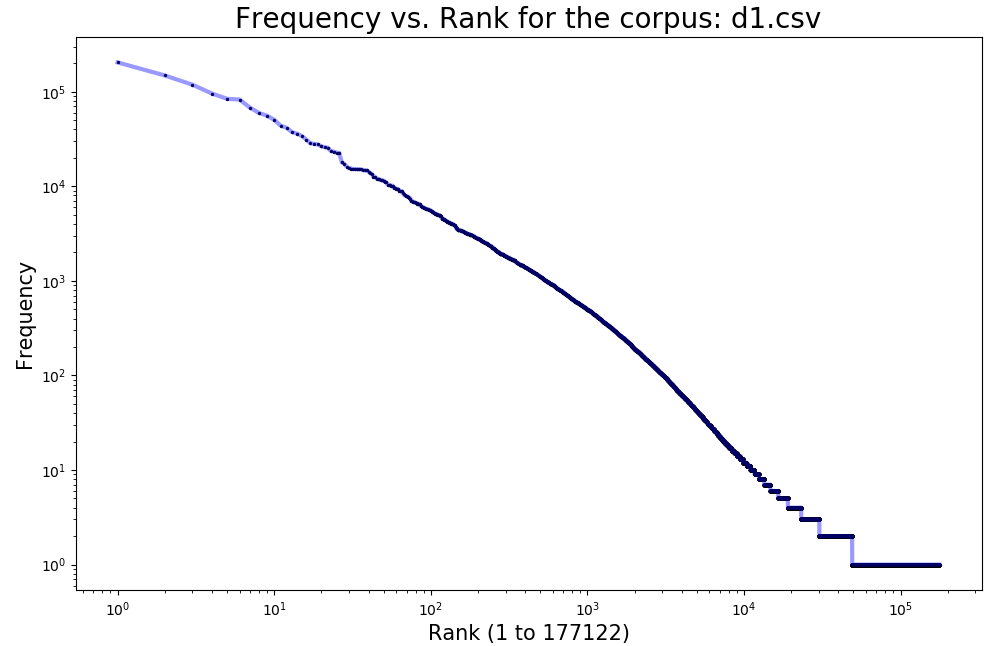
\includegraphics[width=0.75\textwidth]{./images/dataset-1-t1-0.png}
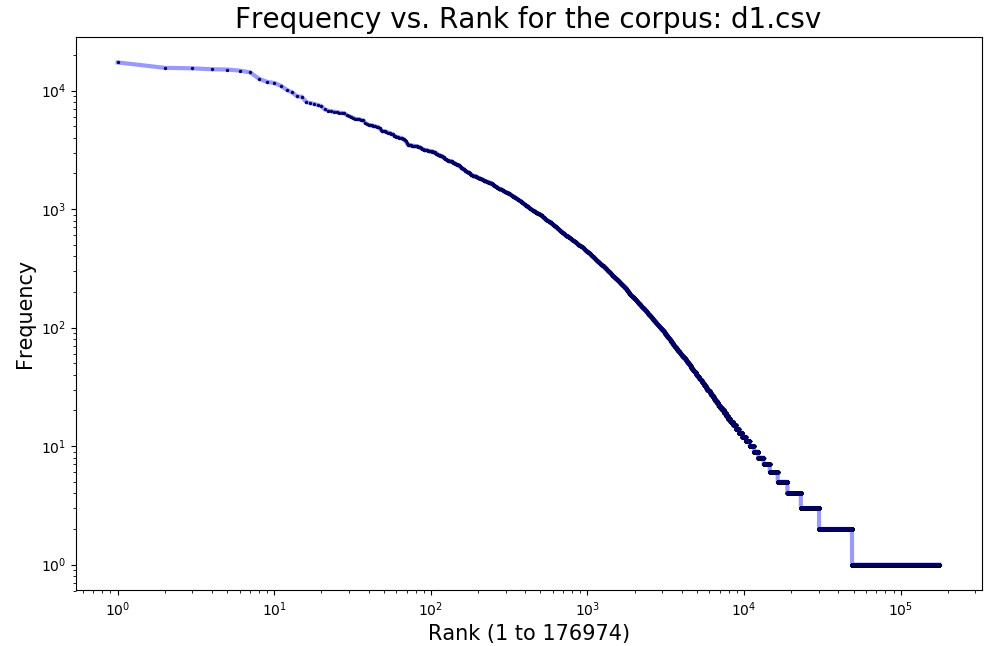
\includegraphics[width=0.75\textwidth]{./images/dataset-1-t1-1.png}
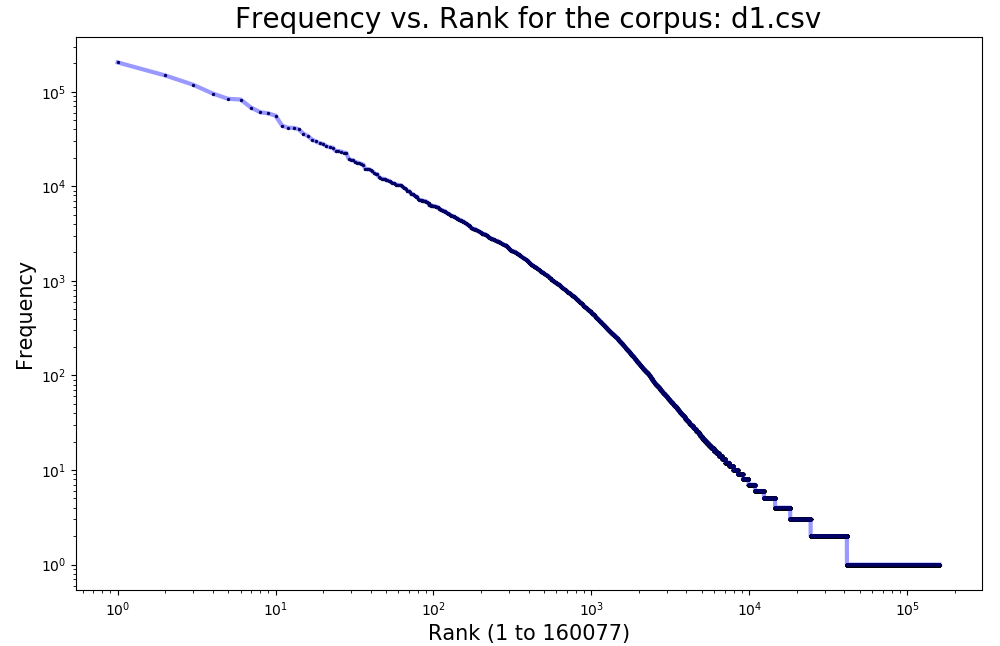
\includegraphics[width=0.75\textwidth]{./images/dataset-1-t1-2.png}
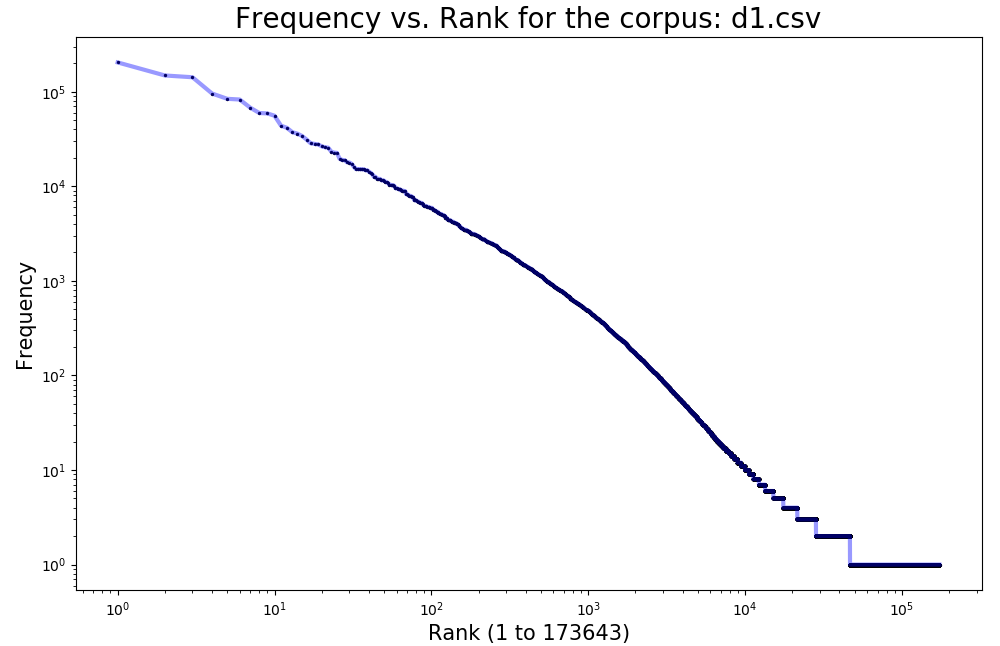
\includegraphics[width=0.75\textwidth]{./images/dataset-1-t1-3.png}
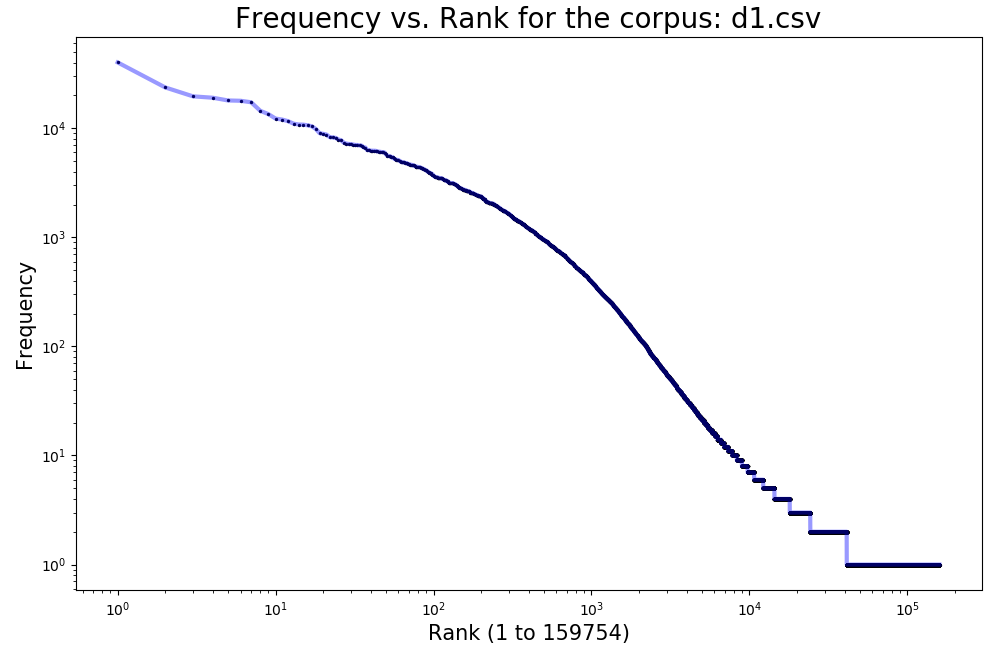
\includegraphics[width=0.75\textwidth]{./images/dataset-1-t1-4.png}
\end{minipage}
\hfill
\begin{minipage}{0.45\linewidth}
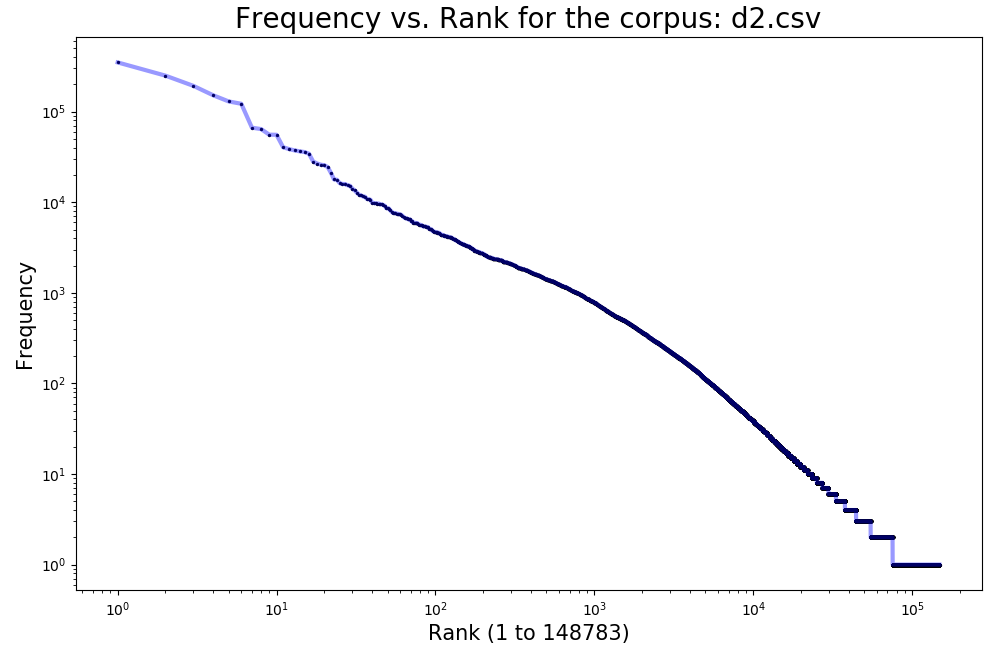
\includegraphics[width=0.75\textwidth]{./images/dataset-2-t1-0.png}
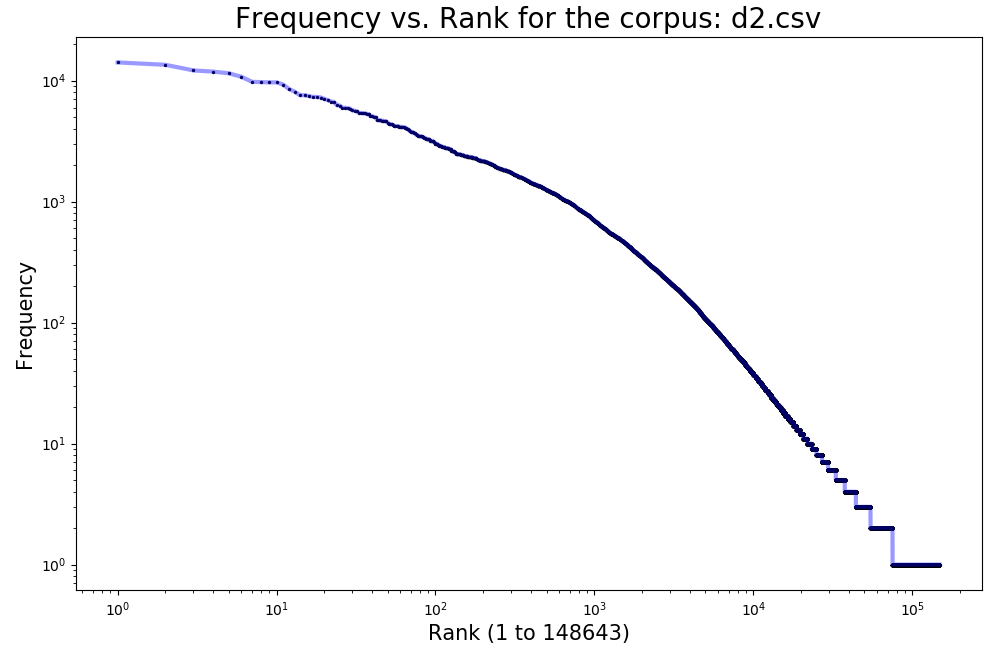
\includegraphics[width=0.75\textwidth]{./images/dataset-2-t1-1.png}
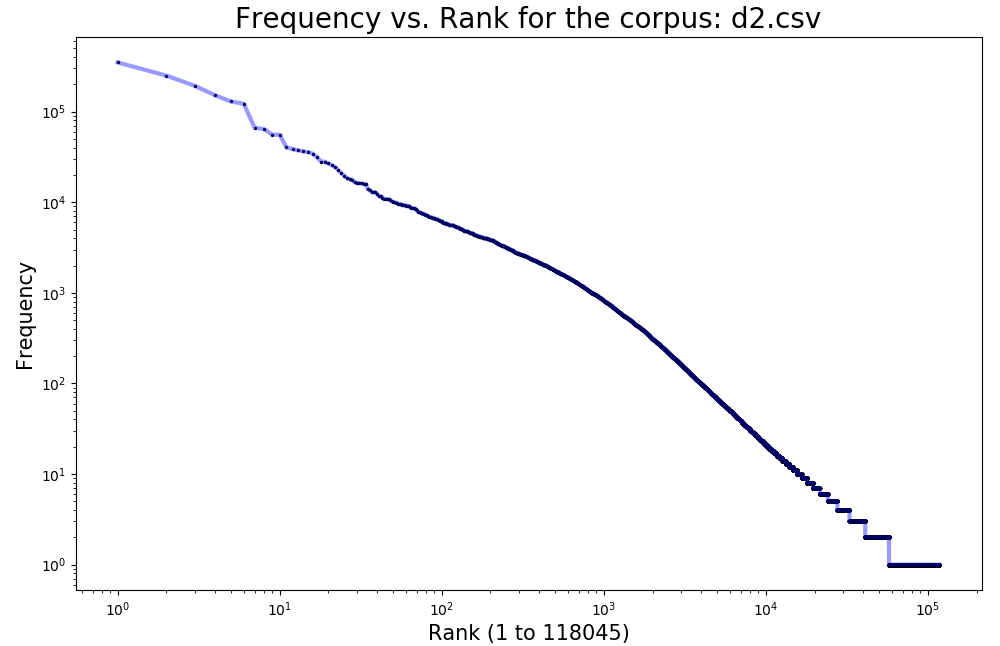
\includegraphics[width=0.75\textwidth]{./images/dataset-2-t1-2.png}
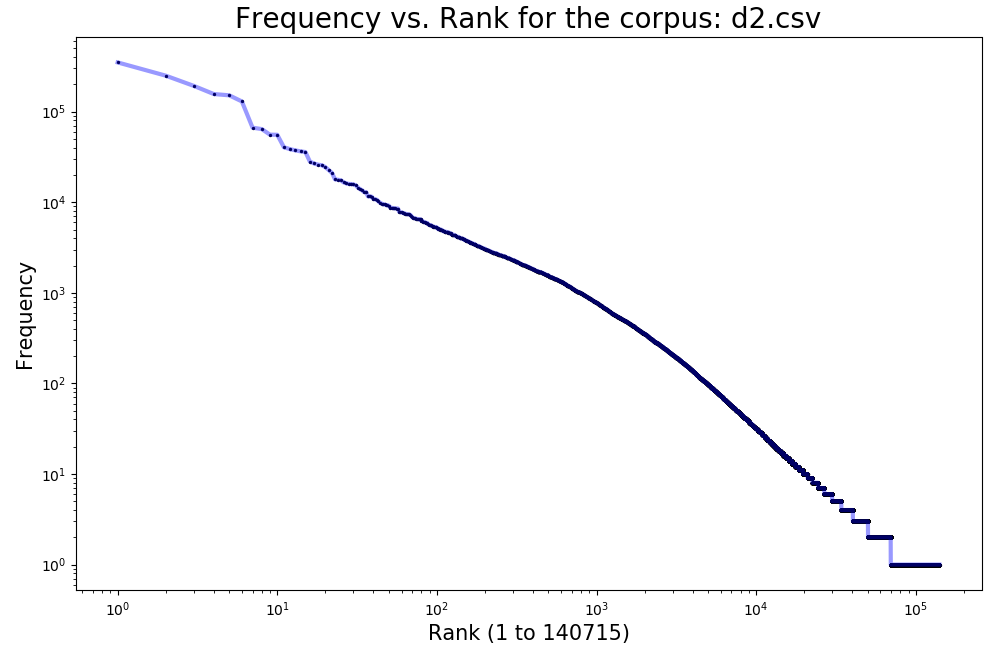
\includegraphics[width=0.75\textwidth]{./images/dataset-2-t1-3.png}
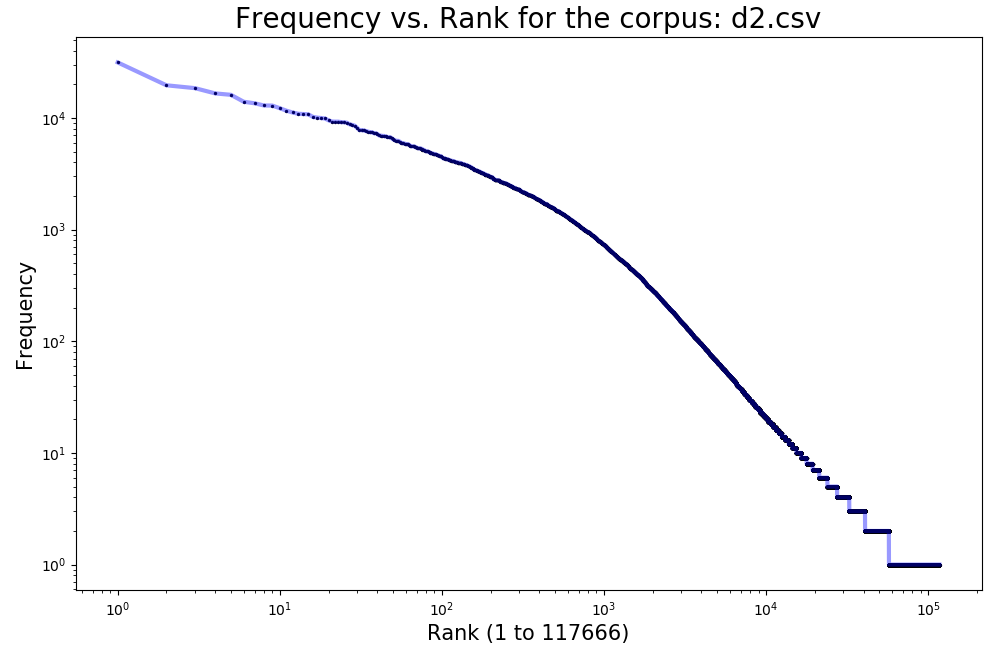
\includegraphics[width=0.75\textwidth]{./images/dataset-2-t1-4.png}
\end{minipage}
\caption{Results for Dataset 1 (Left) and Dataset 2 (Right).\newline{}These are log plots for better visualization. Each plot from top to bottom represents a sequence of processing steps.\newline{}These are (ordered from top to bottom): [1, 2], [1, 2, 3], [1, 2, 4], [1, 2, 5], [1, 2, 3, 4, 5]}
\end{figure}
\end{flushleft}

\subsubsection{Top 20 words}
\begin{flushleft}
The top 20 words obtained after each of the five sequences of processing steps are tabulated below (Dataset 1 on the left, Dataset 2 on the right):
\begin{center}
\begin{tabular}{|p{0.08\textwidth}|p{0.37\textwidth}||p{0.08\textwidth}|p{0.37\textwidth}|}
\hline
Processing Steps & Top 20 Words & Processing Steps & Top 20 Words \\
\hline
\hline
[1,2] & the, to, a, i, is, and, of, that, in, it, for, this, be, on, my, with, can, not, have, or &
[1,2] & the, of, and, in, to, a, is, for, with, that, this, we, on, by, are, as, was, an, be, were\\
\hline
[1,2,3] & would, key, server, using, password, use, security, like, user, im, data, one, know, access, could, way, get, secure, file, used &[1,2,3] & results, data, study, patients, using, also, model, system, used, paper, two, may, one, use, p, analysis, time, different, based, information\\
\hline
[1,2,4] & the, to, a, i, is, and, of, that, it, in, for, be, thi, use, on, my, with, have, can, not &
[1,2,4] & the, of, and, in, to, a, is, for, with, that, thi, we, on, by, are, as, use, wa, be, an\\
\hline
[1,2,5] & the, to, a, i, is, and, of, that, it, in, for, this, be, on, my, with, can, not, have, or &
[1,2,5] & the, of, and, a, in, to, is, for, with, that, this, we, on, by, are, wa, an, be, were, from\\
\hline
[1,2,3,4,5] & use, secur, password, key, server, user, would, encrypt, like, attack, file, im, data, one, know, access, get, certif, way, could &
[1,2,3,4,5] & use, studi, result, model, system, patient, data, method, effect, differ, cell, present, develop, show, also, paper, function, activ, increas, perform\\
\hline
\end{tabular}
\end{center}
\end{flushleft}
\end{document}
